\begin{savequote}[8cm]
    In the beginning there was nothing, which exploded.
  \qauthor{--- Terry Pratchett, \textit{Lords and Ladies}}
\end{savequote}


% What I have is:
%   Some work on a method for demographic inference (this could be how genetic variation is a marker for demographics)
%   A novel result about a migration (how shared genetic variation can be used as information to determine history)
%   Shared genetic variation across the genome can show transcription factor networks 
%       but we haven't really shown this.
% 
%   A good way to phrase this is that I want to use machine learning and statistical inference
% methods to leverage the variation between genomes to solve outstanding problems in 
% statistical genetics, and try to integrate over the variation within the genome to understand
% to identify regulatory structures for a particular disease with a single genetic difference.. 

% So in the introduction I can talk about 
%       - What causes genetic variation between individuals
%           - What models we have for how this occurs (coalescent, generating models)
%       - How can we use variation within the genome to facilitate functional genomics?
%           - In this case, variation is much more like noise, and we have to see through it 
%               to get at biological pathways. 
% The general idea is to use machine learning to wrangle genetic variation into patterns which can be used to inform
% the pursuit of understanding biology. 
%
%
%
% Outline (goal of about 20-25 pages I guess). 
% It can be both informative and a source of noise in statistical models which seek to simplify
% to usable results.
%
%   First, need to establish the problem. What is the problem?
%       The problem is that the genome is hugely important for understanding 
%       how the human body functions at a molecular level. When things go wrong,
%       the result is disease. Some of the answers for how and why disease occurs can '
%       lie in figuring out molecular mechanisms that are disrupted by disease.  
%  and again the answers for what cuase the disease can 
%       sometimes lie in what went wrong with the genetics. Understanding how the genome is
%       organised, and how the actual sequence of base pairs relates to biological processes
% 
%   But this isn't exactly a good lead in for the second part of the thesis. The question there is more
% can we group accessible elements which are important for leukemia. Then how can we uncover the 
% similarities in these and find out what is happening on a molecular level. 
%   How can the sequence of uniquely accesible elements help us to find out what is happening in cancer?
%       So it's more like machine learning can find patterns in the sequences 
%       but the machine learning is actually just the grouping part, I'm not saying anything about the 
%       actual sequences with that. 
%       So I'm using machine learning to identify accessible sequences that are predominantly associated with
%       the leukemia samples. Does this have to do with genetic variation? Or what can I call this?
%       
%        Okay so MLL is a cancer caused by a single genetic mutation. This single mutation
%        has caused it to go from being a normal cell to being a cancerous one. What happens in the 
        % middle between the single mutation and cancer?
% 
        % Can we identify regions of the genome that are associated with the disease?  What does this have to do with Genetic variation?  
            % need a method 
%

% Okay let's try again.
%
%   Two sides of the thesis. Genetic variation between individuals and the effect of genetic variation within a single genome. For the second, take the simplest model system of a single variation. This allows us to ask all sorts of questions about the extent to which a single abherant protein can have on the regulatory structure of the entire genome, and to see how far reaching and connected these things are. One major facet of this regulation that we know about is chromatin accessibility. Can we use machine learning to identify accessible regions of DNA associated with the mutation? 
%   So what do I need to introduce?

    % This is based off of Aaron's framework
    
    % Introduction:
    %     Genetic variation causes
    %     Genetic variation between individuals and coalescent theory
    %     Impact of genetic variation within the genome: a chromosomal translocation event and mixed lineage leukemia.
    %         - 

    % Part 1: Interpreting genetic variation between individuals 
    %     Chapter 1: A particle filter for demographic inference
    %     Chapter 2: Ancient admixture 
    % Part 2: The impacts of genetic variation within a single genome
    %     Chapter 3: LDA for bulk ATAC-seq and Erythropoesis
    %     Chapter 4: LDA for MLL-r 
    %     Chapter 5: A NN for blah
    % Part 3: End matter

    % For the MLL part:
    %     Genomic regulation by chromatin conformation and accessible DNA.
    %         How is it regulated? What are the effects?
    %         Measuring it via ATAC-seq and DNA-ase seq
    %     Topic modelling (I can save this for the chapter)
    %         General idea
    %         LDA 
    %         Adjusting the algorithm for bulk ATAC-seq. (This is due to a lack of appropriate differentiation systems for single cell. )
    %     MLL leukemia biology and pathology (This can be )
    %         Also will need to introduce erythropoesis too if this will be a big part of it.
    %         Will this be a seperate chapter? Or a part of the topic modelling chapter?

    %     * My big problem is that this isn't really related to genetic variation.... It's more
    %         like finding regions associated with a cell type. 


    % page counts...
    %   intro: 10
    %   1: smc2 - 20 pages
    %   2: bm - 30 pages
    %   3: ery: 25 pages
    %   4: mll: 25
    %   5. condlusion : 10


% Introduction Outline: 

% \begin{itemize}
%     \item Genomic Sequencing Data
        
%     \begin{enumerate}
%         \item Enabling advances in Sequencing technologies
%         \item Applications of sequencing technologies
%         \begin{enumerate}
%             \item Whole genome sequencing enables us to study population variation across the globe.  (whole genome sequencing)
%             \begin{enumerate}
%                 \item Technical error and variant calling
%                 % I dont deal with this but its an important caveat
%                 \item Issues with assembly in diverse populations
%             \end{enumerate}
%             \item Functional genomics (ATAC-seq, DNAse-seq, ChIP-seq, etc.)
%             \begin{enumerate}
%                 \item 
%             \end{enumerate}
%         \end{enumerate}

%     \end{enumerate}

%     \item Machine Learning and Statistical Inference for sequencing data
%     \begin{enumerate}
%         \item Reasons for considering machine learning for these two problems.
%     \end{enumerate} 
     
%     \item \textbf{Aim}: Use sequencing data and machine learning to find new ways to answer outstanding issues at the population and cellular scale.
%     \begin{enumerate}
%         \item \textbf{Specific Aim 1}: Estimate a coloured ancestral recombination graph from WGS Data
%         \begin{enumerate}
%             \item Modelling ancestry with the coalescent
%             \item Traditional approaches to modelling demography
%             \item Sequential Monte Carlo
%             \item Advantages, including directional migration
%         \end{enumerate}
%         \item \textbf{Specific Aim 2}: Predict Regulatory Regions of MLL-AF4 Leukemia from ATAC-seq
%         \begin{enumerate}
%             \item Traditional methods for genomic sequence annotation
%             \item Artificial Neural Networks
%             \item Adopting artificial intelligence models for sequence based learning
%             \item Advantages , including in silico mutagenesis 
%         \end{enumerate}
%     \end{enumerate}
% \end{itemize}

\chapter{\label{ch:1-intro} Machine Learning and Next Generation Sequencing} 

%\minitoc

Genomics has taken front and centre stage recently in the search for knowledge about our physiology and our humanity. Much of this growth from the time of Mendel's peas to the current era of rapid development and global vaccination against deadly disease with messenger RNAs has come at the heels of technological developments in sequencing technologies. As we continue to explore the questions raised by the first efforts to understand what it is that makes up humanity at a molecular level, the availability of massively high-throughput sequencing has allowed for the study of our species, from its history to its pathology. Cost lowers every year, and with it, so too does the barrier to entry into genomics research. This explosion in sequencing data, concurrent with a famously exponential increase in computational processing power, has changed the way that we conduct research and philosophically approach hypothesis testing. Alogirthms designed to learn patterns directly from petabytes of freely available data prioritize biological hypotheses. This thesis broadly aims to extend the use of machine learning for next generation sequencing data in two different ways. Firstly, by learning demographic parameters from whole genome sequencing data, and secondly by learning cellular regulatory programs from collections of accessible chromatin experiments. We apply the first method to detect a substantial back migration in the ancient past, and the second to identify a subset of novel enhancer elements active in childhood KMT2A-AFF1 leukemia patients. These methods both address open questions in the field, and provide novel insight into human origins and the dysregulation of functional genomics leading to cancer.

This chapter is structured as follows. I begin by introducing next generation sequencing and its development. Next, I give context to the long-standing problem of demographic inference and how the NGS revolution has set the stage for the use of large-scale machine learning algorithms. I also briefly describe the mathematical model underpinning these methods and other comparable approaches. We then pivot to discussing the application of next generation sequencing to functional genomics and the development of \gls{atac}, \gls{chip}, and RNA sequencing. I describe previous approaches for learning from these data applied to childhood leukemias and more broadly. 


\section{The Evolution of Next Generation Sequencing}

The order of bases in poly-nucleotide chains simultaneously encode the instructions for protein synthesis and all information about the geneological history of an individual. Despite an understanding of the three-dimensional structure of \gls{dna} in the early 1950s, the first protein-coding gene sequence was not completed until 1972 \cite{JD1953,JOU1972}. By this point, a sequencing method developed by Fred Sanger and colleagues was giving rise to the first generation of sequencing technologies \cite{Kulkarni2014}. Sanger sequencing, and its more modern incarnation Sanger sequencing by capiliary electrophoresis, remains an important technique for clinical genomics and is the gold standard for accuracy \cite{Shendure2017}. This thesis is concerned with the analysis of data resulting from sequencing technologies, and not the mechanism of sequencing itself, so descriptions here will be brief. Sanger sequencing combines denatured single-stranded DNA molecules and a solution of nucleotides with small amounts of chain-terminating dideoxynucleotides to produce fragments of varying lengths, which can then be separated by molecular weight through electrophoresis and read either manually from a slab gel or automatically through a capillary \cite{F1977,Liu2012}. Modern iterations are capable of processing up to X samples concurrently, improving substantially over previous iterations of the technique which required manual base calling (Cite Illumina). 

In many ways, modern NGS techniques are natural extensions of the original Sanger sequencing method. The first step in an NGS workflow is library preparation \cite{Head2018}. This step involves gathering DNA or \gls{rna} from the experimental design being employed, such as \gls{wgs}, fragmenting the product to a desired length and attaching oligonucleotide adaptors to both the 3' and 5' ends of the sequence. Adaptors are attached either through ligation, where adaptors are ligated to end-repaired inserts, or by "tagmentation" where a single transposase enzyme fragments and ligates adaptors in a single step \cite{R2011}. Preparing and assessing the quality of a library is a crucial step in the process of NGS, and much literature is dedicated to an exposition of the subject (CITE). 

\subsection{Next generation sequencing methods} \label{intro:ngs_methods}

There are two main methods for \gls{srs} currently available on the market. These include: 

\begin{enumerate}
    \item \Gls{sbs} is used by technologies like Illumina Novaseq 6000. After library preparation, fragmented sequences with annealed primers are allowed to hybridize to fixed anchor sequences on the surface of a glass sequencing chip. In a process called bridge amplification the reverse primer anneals to an adjacent anchor sequence and polymerase enzymes synthesize the original fragment of DNA. The bridges are broken to form single stranded sequences, and the process is repeated to form clusters of clones, each representing a single fragment of the original fractionated DNA. Reversibly-terminated fluorescently-labeled nucleotides are incorporated to the solution, and the sequencing chip is imaged to determine the consensus nucleotide incorporated for each cluster of fragments. The termination domain is washed away and the process repeated for a given insert length. Additions to this protocol can include a subsequent step where partial bridge amplification followed by the synthesis reaction sequences the insert from the 5' rather than the 3' end and the incorporation of sample specific or microfluidics-based barcodes which encode the source of the insert. Protocols for sequencing by synthesis are taken from \textcite{Illumina}.
    \item \Gls{sbl} is primarily used in SOLiD sequencing from Life Technologies and shares many similarities with sequencing by synthesis, including the preliminary fractionation, annealing of sequencing primers, and hybridization wth anchors on the surface of the sequencing chip. Rather than allowing individual bases to join the single stranded insert, however, sequencing by ligation allows DNA ligase enzymes to join entire nucleotides, relying on the reduced efficiency of the ligase for mismatching sequences. These labelled oligos are fluorescently dyed and when imaged provide information on several of the first bases in the unknown sequence of the insert. Depending on the specific protocol, oligose are cleaved and the process repeated outwards from the anchor sequence. Details of the sequencing protocol were taken from \textcite{Slatko2018}.
\end{enumerate}

Other sequencing methods exist for specific situations, and have been categorized into "third" and "fourth" wave depending on their capabilities \cite{Slatko2018}. A notable example is Oxford Nanopore sequencing, which is able to provide long reads theoretically up to hundreds of kilobases and is currently suitable for resolving structural variants \cite{AByrne2019,Bayega2018}. The per-base error rate is higher than with SBS or SBL techniques, but this is steadily improving year over year \cite{Sahlin2021}. These new and evolving techniques have an extensive literature dedicated to their uses and applications, which are not within the scope of this brief review or this thesis, but show huge promise for future applications in population and functional genomics. 

After imaging each of the clusters on the flow cells, both protocols must identify nucleotides and their associated confidence in a process known as base calling. The result is a collection of similarly sized contiguous "reads" from the unknown DNA, each annotated with its sequencing primer and optionally a barcode with additional information about the sample that it derives from in the case of library multiplexing. The next steps in analyzing NGS data are almost entirely computational, and differ between sequencing applications. In general, these steps aim to filter and control the resulting base calls such that errors in analysis due to sequencing artifacts are minimized. These include, but are not limited to, errors in base calling and small \glspl{indel}, poor quality reads, and adaptor or sequencing primer contamination in the final data \cite{Slatko2018}. Tools such as FastQC provide an accessible interface for performing common quality control procedures on raw data from sequencing platforms, assessing and marking reads which fail per-base and per-sequence error-rate, quality metrics, GC-content, length, segment duplication, and kmer counts \cite{Andrews2015}. These marked reads can be removed along with sequencing adaptors using Trimmomatic or CutAdapt among others \cite{Martin2011a,Bolger2014}. This previously esoteric process has been greatly simplified in recent years due to large amounts of work from software developers, expanding the accessibility of NGS technologies to areas which have otherwise not been focused on the use of command line tools. The last major step before the procedure branches off to application specific analysis involves identifying the likely origin of each fragment of DNA from the human genome. With equal and independent base probabilities, the chance of observing a particular sequence of length $n$ is simply $\left( \nicefrac{1}{4} \right)^n$ leading to surprisingly specific mapping of fragments to the reference genome by well known algorithms such as the burrows-wheeler aligner (BWA) and bowtie among others \cite{Langmead2009,Li2009}. These computational steps represent a minimal path to usable sequencing reads for further analysis, however each one of these steps involves critical analysis of the data and interpretation that is not the subject of this review.

From this point onwards, we separate the discussion of sequencing technologies and associated machine learning techniques into two sections relevant to the two applications discussed in this thesis.

%\section{Machine Learning and Statistical Inference Methods}

%
%\begin{enumerate}
%    \item 
%\end{enumerate}

%These 


%These methods have been used extensively to study both functional genomics and population genetics. In the following two sections, we explore the use of machine learning within these two fields.  

%The focus

\section{Modern Human Origins and Whole Genome Sequencing}

Recently, the decreased cost and increased availability of \gls{wgs} technologies has allowed for the study of populations previously unrepresented in the genomic record \cite{D2019,Wong2013,Wu2021,GS2019,Fan2019a}. At the same time, mathematical descriptions of how mutations arise and spread within populations have allowed for the development of algorithms to infer influential aspects of the origins, dispersal, and interactions of \glspl{amh} throughout history \cite{Hodgson2010}. Here I introduce the fundamental background necessary to understand how the mathematical modelling of ancestry has allowed for demographic inference from whole genomes. 

% Outline
% Brief description of coalescent theory and its goals

\subsection{A Model to Describe the Evolution of a Sequence}

The Mendelian transmission of genetic material from parent to offspring encodes a record of all ancestral events written in a string of four bases. This process can be modelled by the coalescent, a mathematical formulation of genetic ancestry that makes predictions about patterns of variation as a consequence of a series of unobserved trees along the genome of an individual called the \textit{gene geneology}. Introduced in a series of seminal papers by Kingman, Hudson, and Tajima in the early 1980s, the coalescent is a stochastic process describing the $n-1$ \textit{coalescent} events where lineages from a population of size $n$ find their common ancestor backwards in time until only a single lineage called the \gls{mrca} remains \cite{Hudson1983,Kingman1982,Kingman1982a,F1983}. In contrast to the classical population genetics that dominated the early 20th century, coalescent theory is mostly concerned with a retrospective view of ancestry backwards from the current generation \cite{Ewens1990}. In the simplest case of the original coalescent formulation, it can be shown for reasonable assumptions that in the limit of population size $N$, a time to coalescence for a pair of lineages is exponentially distributed with a mean of 1. The times for each lineage to coalesce (in units of generations) are independent and exponentially distributed as $$ \begin{aligned} f_{T_i} (t_i) &=  \binom{i}{2}  e^{- \binom{i}{2}}  &t_i \geq 0 \end{aligned}$$ for $i = 2, \ldots, n$ and approximates the Wright-Fisher forward-in-time models in this same limit (derivations found in \textcite[Chapter 3.2]{Wakeley2009a}). The coalescent provides an elegant framework to describe the relative likelihood of the marginal trees at each position of the genome given information about genetic variation in a population, however the standard coalescent has proved not powerful enough for many applications. Motivated by the observation of autocorrelation in allele frequencies along the genome, also known as linkage disequilibrium, the importance of recombination in the human genome motivated \textcite{Griffiths1997a} to extend the gene genealogy to include breakpoints where the marginal trees are permitted to change due to potentially differing ancestral origin for each haplotype in a model called the \gls{cwr}. The resulting latent data structure of piecewise constant genealogical trees along the genome, broken up with ancestral recombination breakpoints, is known as the \gls{arg}. The ARG is an explicit representation of the structure underlying empirical \gls{ld} and both represents a record of the ancestral process for each marginal tree and provides information for the mutational process. The ability to infer this data structure represents one of the overarching goals of modern population genomics.  

\subsection{Whole Genome Sequencing for Population Genomics} \label{intro:popgen}

For the majority of the twentieth century, population genetics was driven by developments in mathematical modelling rather than insights from real data. This situation changed radically as the scale of data grew exponentially as \gls{pcr} and small-scale DNA-sequencing, polymorphism data, and finally population level sequencing experiments shifted the focus of the field to be primarily driven by data \cite{Kreitman1983,JE2010,Crawford2012}. Though analyses based on \glspl{snp} are still a mainstay in the field (i.e. many studies have used, adapted, and extended the formal statistical methods for the analysis of genome-wide polymorphism data presented in \textcite{Patterson2012a} such as \cite{Skoglund2017,Durand2011,Lipson2017,Skoglund2015,Pickrell2012,Wall2000,Nielsen2017a,Carto2009,Margaryan2020}), many recent efforts focus on the use of \gls{wgs} to accurately survey the distribution of genetic variation across global populations and even ancient humans such as Neanderthals \cite{Fan2019a,Mallick2016,Prufer2014,Bergstrom2019, Auton2015}. WGS presents several attractive properties over polymorphism data for population level genetics \cite{Hoglund2019}. Most obviously, the ability of WGS to discover not only selected and imputed variants but all variation in the genome is both an advantage for population genetics and a disadvantage for medical genomics, with some early indications that the cost efficiency and increased multiple testing burden may support whole exome sequencing for the discovery of functional variants \cite{Lacey2014}. This, however, is beneficial to demographic inference and many coalescent based approaches which assume selectively neutral loci. An additional benefit is the ability for researchers to move beyond the standard reference panel and identify structural variation and private polymorphisms in understudied population such as South Africans \cite{Choudhury2017a}. Though these analyses are technically challenging, a clear understanding of the actual structure of the genome for specific populations can help to avoid unnecessary read mapping artefacts and better represent the underlying evolutionary process. 

Methodologically, \gls{wgs} typically follows the steps laid out above \Cref{intro:ngs_methods}, however an important aspect to consider with regards to population genomics analyses is the phasing strategy employed. Humans are diploids, meaning that one set of chromosomes is inherited paternally and the other maternally. At its core, the NGS protocol does not phase, or delineate the nucleotide content of the two sets of chromosomes. Estimating the phase of sequence variation is a critical step in many population genetics pipelines as single pieces of individual genomes (haplotypes or haploblocks) are passed down from generation to generation. There are many strategies for estimating the phase of a sequence (\textcite{Choi2018} studied and compared eleven such methods with regards to a single well-characterized genome), however experimental phasing strategies such as those employed in a subset of the the dataset presented in \textcite{Bergstrom2019} (the \gls{hgdp}). \textcite{Bergstrom2019} employed a linked-read sequencing technology based on microfluidics to computationally reconstruct long haplotypes and structural variants (method is adapted from \cite{GX2016}). As the authors note, however, long read sequencing may enable cheaper, faster, and more accurate resolution of phase in diverse populations in the future. Other studies have opted for the approach of using statistically phased genomes in their analyses despite the known bias in parameter estimates as a consequence of errors in statistical phasing (see \textcite[Supplemental section 7]{Steinrucken2019} and \textcite{Raghavan2015a} for a simulation study which explores this). \textcite{Choi2018} optimistically found that a combination of computational strategies are able to approach experimental levels of accuracy without the need for expensive re-sequencing, so it is likely that in the near future a combination of innovation in long read sequencing and statistical phasing methods will ameliorate the systematic issues caused by inaccurate phasing in demographic inference. Phasing and its accuracy is an important factor to consider when interpreting the inferred parameter values from machine learning methods which aim to infer demographic parameters and the ancestral recombination graph as a whole.

\subsection{Using Machine Learning to Infer the Ancestral Recombination Graph from WGS Data}

% SMC 
Stochastic simulation under the \gls{cwr} model backwards in time is computationally efficient, as the generational coalescent and recombination rates are simple a Markovian function of the ancestral lineages present in that generation \cite{RR1983}. However, for reasons of computational efficiency, in many applications it is desirable to simulate trees along the genome rather than in time. Under the CwR model, the marginal trees along the genome have a complex, non-Markovian relationship, with each tree depending on every tree preceding it in the sequence \cite{C1999}. A desire for a computationally tractable method for simulating genologies along the genome lead \textcite{McVean2005a} to extend the work of \textcite{C1999} to develop a Markovian approximation of this process called the \gls{smc}, greatly simplifying the problem of demographic inference along the genome and leading to the first true inference algorithm for piecewise constant population size inference known as the \gls{psmc} \cite{Li2011a}. The key innovation put forward by PSMC was to approximate the continuous state space for the Markov chain with a more reasonably size finite set of topologies and discretised time intervals where coalescent events may occur. Inference is then performed with a \gls{hmm} over pairs of chromosomes in the samples, estimating the piecewise constant ancestral coalescent rates given a fixed mutation and recombination rate. The coalescent rate in a particular era is inversely proportion to the ancestral population size at that point in time, making the \gls{iicr} a reasonable estimator for the effective population size ($N_e$) in pan-mictic populations \cite{Chikhi2018}. In this way, the \gls{hmm} functions as a machine learning model using the observed mutations to maximize the probability of generating the inferred tMRCAs given a specific set of coalescent rates discretized over time. With an explicit and tractable likelihood function to work with, modern machine learning and statistical inference methods such as \gls{msmc} (with extensions such as MSMC-IM) have become gold standard approaches for studying the deep histories of global populations through their inferred $N_e$ \cite{Wang2020,Fan2019b,Schiffels2014c}. At the same time, machine learning methods are moving beyond summaries of the underlying data (such as the tMRCA, \gls{sfs}, principle component analyses, and haplotype maps) to inferring the entire underlying ARG for a group of samples. The first method to do so on a genome-wide scale was ArgWeaver, which used a \gls{mcmc} sampler to asymptotically sample from the posterior distribution of single panmictic population ARGs conditioned on observed genetic variation, assuming a single population in panmixia \cite{Rasmussen2014a}. An extension of this method, ArgWeaver-D is also capable of inferring ARGs from WGS data conditioned on a user-specified topology, including migration, however it requires a fixed topology from which to effectively infer branch lengths \cite{Hubisz2020}. Relate uses a modified version of the \textcite{N2003} \gls{hmm} to efficiently construct a distance matrix between samples in the dataset; a tree is constructed from this non-symmetrical distance matrix and branch lengths are estimated using a coalescent-aware MCMC \cite{Speidel2019a}. A different approach is taken by tsInfer, which uses a heuristic algorithm to infer ancestral haplotypes and their most likely path to the current haplotypes through an error-prone copying process \cite{Kelleher2019a}. These three examples represent the current gold standard machine learning algorithms to maximise the likelihood of a set of marginal trees given observations about genetic variation.

\section{Functional Genomics and Machine Learning} \label{intro:fungen}

Another aspect of the field impacted by advancements in NGS technologies is functional genomics. Concerned with deciphering the genomic code by which genes and their networks are regulated, NGS techniques have allowed for the efficient profiling of transcription and epigenetic processes with unprecedented resolution \cite{Morozova2008,Cullum2011,Morozova2008a,Hurd2009,T2010}. As research groups and consortia are increasingly sharing their data publicly using tools such as the Gene Expression Omnibus (\url{https://www.ncbi.nlm.nih.gov/geo/}) and the Sequence Read Archive (\url{https://www.ncbi.nlm.nih.gov/sra}), massive amounts of data on many different cellular systems are now freely available. Tools are needed to simplify and reduce the dimensionality of these datasets so that expert knowledge can be used to understand the biological processes underlying them. This section introduces the fundamental NGS techniques used in functional genomics (as relevant for this thesis) and how machine learning is being used to draw biological insight from them.

\subsection{NGS-based Functional Assays}

NGS techniques have been adopted to study many facets of a cell's genome, usually by strategically fragmenting the sequence to predominantly represent regions of interest. Here I discuss two individuals techniques that detect chromatin accessibility and protein-DNA interactions.  These assays have direct relevance to the analyses performed in this thesis. There exist more techniques that are not discussed here, or which are introduced in this thesis where relevant. 

\subsubsection{Assay for transposase-accessible chromatin with high throughput sequencing} \label{intro:atac}

In 2015 \textcite{Buenrostro2015a} introduced \gls{atac} (\Cref{fig:atac}). The goal of the method is to assess the substantial heterogeneity in physical compaction of the genomic sequence, referred to as chromatin accessibility \cite{Thurman2012a}. Chromatin is a complex of DNA and proteins used to organize the genome, and its fundamental unit is the nucleosome \cite{Bell2011a}. The nucleosome is a complex of DNA wrapped around a protein octamer of four core histones numbered as H2A, H2B, H3, and H4 \cite{Bell2011a}. These histones are frequently the target of post-translational modifications which confer additional functional information about the sequence, as described in the next section on ChIP-seq. In general, a higher density of nucleosomes along a sequence leads to more compact DNA within the nucleus \cite{Kornberg1974}.  
The physical compaction of DNA, a necessary process due to the almost two meters of DNA packed into a five micron nucleus, has been shown to be a key factor in the regulation of transcription by either allowing or blocking transcriptional machinery physical access to the sequence \cite{Bell2011,Gross2003}. A more thorough exploration of chromatin accessibility as it relates to the topics explored in this thesis is presented in the introduction of Chapter 3 in \Cref{ch3:chrom_acc}. 

\begin{figure}
    \centering
    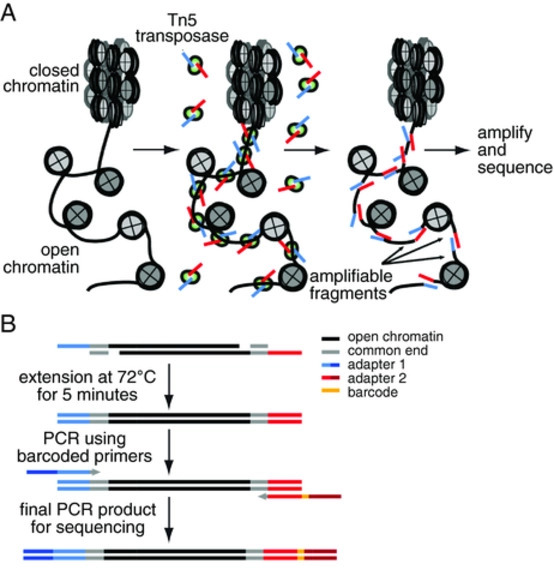
\includegraphics[width=0.5\textwidth]{plot/ch1/atac.jpg}
    \caption{ATAC-seq protocol schematic adopted from \cite{Buenrostro2015a}}
    \label{fig:atac}
\end{figure}

The ATAC-seq assay is conceptually a simple adaptation of the typical NGS procedure, and as previously mentioned relies on strategic sheering of the genome (in this case, targetted amplification) followed by sequencing. Here, a hyperactive Tn5 transposase enzyme preferentially accesses the sequence not wrapped in nucleosomes, inserting sequencing adaptors that can be directly amplified. This results in fragments of DNA whose length follows a bimodal distribution, with the majority derived from the space between nucleosomes and tending to be short, and the minority spanning a nucleosome and thus having a fragment length of at least $\sim$150 base pairs \cite{Yan2020a}. Since the amplified pieces of sequence predominantly appear in regions without nucleosomes, identifying "accessible" regions (for a given threshold) is an exercise in statistical detection of regions with signal enriched over the background.

The concept behind ATAC-seq is similar to previous assays for chromatin accessibility such as MNase-seq and DNAse-seq which use micrococcal nucleases, and DNAse 1 enzymes to fragment the sequence respectively \cite{Bell2011a}. FAIRE-seq, a successor to DNAse-seq introduced in \textcite{Giresi2007}, performs a fundamentally different fragmentation by isolating DNA that is not able to be experimentally cross-linked to nucleosomes. In contrast to MNAse-seq and DNAse-seq, ATAC-seq requires far fewer experimental steps and isolated cells, allowing for efficient study of small populations of cells (as shown by \textcite{Buenrostro2015a}) while comparisons with FAIRE-seq show substantial bias in the latter towards enhancer and intronic elements and a smaller enrichment of signal over the sequencing background \cite{Tsompana2014}. This makes ATAC-seq an experimentally efficient procedure for generating high coverage chromatin accessibility tracks in low to moderate numbers of cells. DNAse-seq was adopted enthusiastically by consortia such as \textcite{ENCODEProjectConsortium2012} and substantial effectively-legacy data exists from this assay, however more recent efforts in the same groups (i.e. \textcite{Moore2020}) are focusing on ATAC-seq for this task. The analysis of ATAC-seq data therefore remains a valuable task, especially as the number of generated datasets continues to increase year over year (\textcite{Yan2020a} demonstrates this up until 2019).

\subsubsection{Chromatin immunoprecipitation followed by sequencing} \label{intro:chip}

Both the combinatorial binding of transcription factors and post-translational modification of histone proteins are key players in the complex logic of gene expression \cite{Farnham2009}. Transcription is regulated by a large number of \glspl{cre} categorized by function and distance to the \gls{tss}. These include promoters and promoter-proximal elements, enhancers, silencers, insulators, and boundary elements for topologically associated DNA domains (reviewed in \textcite{Wittkopp2011}). Many transcription factors bind to specific patterns in DNA called ``motifs'', however the majority have either a non-specific binding sequence or none at all, leading to the desire for an experimental approach to determine where specific transcription factors are bound in specific cellular contexts \cite{Spitz2012}. At the same time, specific covalent modifications to histone proteins have been shown to be enriched at active enhancer and promoter elements, indicating their involvement in the recruitment of proteins for transcriptional activation. For the purposes of this thesis, only a handful of the many histone modifications are necessary for the putative identification of enhancer and promoter regions (\Cref{fig:histones}). In the following and throughout, the nomenclature for histone modifications is the histone that is modified (Histone H3 = H3), the residue that is modified (lysine residue 4 = K4), and the actual modification (me1 = mono-methylation, me3 = tri-methylation, ac = acetylation) such that, for example, mono-methylation of the fourth lysine residue on histone protein H3 would be denoted as H3K4me1 \cite{Gates2017}. A summary of important histone modification follows.

\begin{figure}
    \centering
    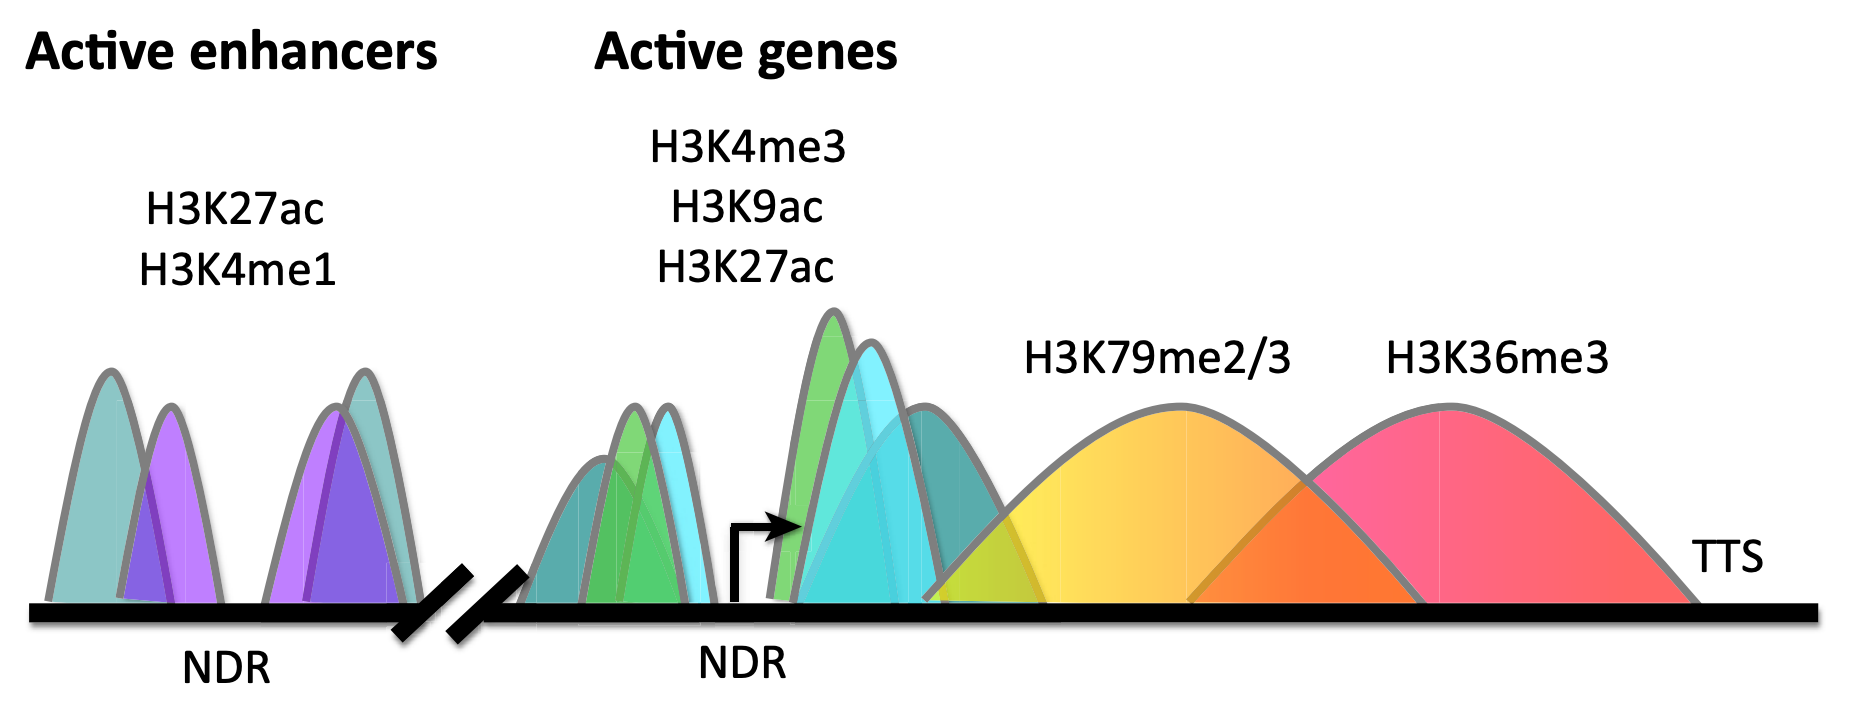
\includegraphics[width=\textwidth]{plot/ch1/histones}
    \caption{Typical eukaryotic ChIP-seq defined active enhancer, promoter, and gene body histone modifications from \textcite{Gates2017}. H3K4me3 and H3K9ac typically load onto active promoter regions, while H3K79me2/3 and H3K36me3 are found on the actual gene body being transcribed. H3K27ac loads onto both active promoters and enhancers, while H3K4me1 is found predominantly on the latter. These are all generalizations, and represent typically found patterns. NDR = nucleosome-depleted (accessible) regions, TSS = transcription start site.}
    \label{fig:histones}
\end{figure}

\paragraph{H3K4me1} is found predominantly at enhancer elements \cite{Gates2017}. Recent evidence suggests that H3K4me1 can also be found in promoter elements, with a bimodal pattern flanking H3K4me3 in active promoters and unimodal peak, coinciding with H3K4me3 and H3K27me3, proximal to the \gls{tss} in poised promoters \cite{Bae2020}.  

\paragraph{H3K4me3} is typically believed to be the distinguishing mark of promoter elements \cite{Gates2017}. Typically, the dynamic regulation of methylation between DNA methylation, H3K4me1, and H3K4me3 is able to alter to state of a region from functionally inactive to enhancer or promoter elements respectively \cite{Sharifi-Zarchi2017}. Interestingly though, H3K4me3 occasionally is observed on putative ``super enhancers'', especially in some cancers, though this relationship is the subject of much debate \cite{Li2019}.  

\paragraph{H3K27ac} is an activity marker found at both active enhancers and promoters \cite{Gates2017}.

\paragraph{H3K79me2/3} as in, either the di or tri methylation of H3K79, is unqiuely deposited by the \gls{dot1l} protein, and is often found within the body of actively transcribed genes and is associated with transcriptional elongation \cite{DJ2008,Q2002a}. While not usually found at enhancer elements, recent evidence strongly suggests a role for DOT1L mediated H3K79 methylation in enhancer-promoter interactions in cancers caused by \gls{mll} fusion proteins, which is of interest to results later in this thesis \cite{Godfrey2019a}. 

\paragraph{H3K27me3} functions as a repressive mark for gene expression and is found at silencer elements \cite{Cai2021, Gates2017}. 

These marks vary across the genome depending on a large number of biological factors; ChIP-seq provides an empirical tool to measure their presence. 

ChIP-seq combines chromatin immunoprecipitation (ChIP) with NGS sequencing to identify protein-DNA interactions on a genome-wide scale \cite{Park2009a}. ChIP involves the covalent crosslinking of DNA to any associated proteins followed by the random fragmentation of the genome; specific antibodies are used to ``pull down'' regions bound by a specific protein or histone modification, and the remainder are washed away \cite{Nakato2021,Furey2012}. The remaining fragments of DNA are annealed to sequencing primers and amplified. The effect of this procedure is to enrich sequenced regions for areas of the genome bound by a specific protein. Typically, ChIP-seq experiments are paired with an ``input'' run, in which the pull down step is not performed, in order to assess the genomic background of enriched regions. These are typically removed from the analysis and peak calling as they represent technical artefacts and not biologically relevant DNA-protein complexes. 

\subsection{Specific Machine Learning Applications for Functional Genomics}

\subsubsection{Identifying Signal Enrichement (Peak Calling) with Machine Learning}

One of the key tasks after performing ATAC-seq or ChIP-seq is to determine regions which are enriched for signal over the background \cite{Yan2020a}. Many approaches have been developed for this task (partially reviewed and benchmarked in \textcite{R2017}) based on statistical models typically modelling signal to noise ratios according to a Poisson distribution. This model appears to correctly discriminate visually enriched peak regions, though both the false positives and false negative identifications are frequently thought to be bottlenecks in analyses that rely on discretized region sets. Recently, a deep learning based peak called was proposed which appears to exceed the performance of the gold standard approach, MaCS2 \cite{Hentges2021a,Zhang2008,Gaspar2018}. The model relies on a wide-and-deep convolutional neural network trained on a manually curated set of 8463 peaks from various \textcite{ENCODEProjectConsortium2012} datasets and 8503 noise regions \cite{Cheng2016,Hentges2021a}. 

\subsubsection{Chromatin State Annotation}

After sequencing and discretizing histone modifications into peak regions, a researcher may wish to annotate the genome of their cell type of interest with putative states (i.e. active or poised enhancer or promoter, heterochromatin, etc.). Due to the high dimensionality of the data (a number of chromatin marks each with a genome-scale coverage track), this is a difficult task to perform manually. \textcite{Ernst2012} discovered that by modelling the chromatin state along the genome as a Markovian process, inference of putative states can be efficiently performed with standard approaches such as \glspl{hmm}. ChromHMM and extensions have remained standard approaches for chromatin state annotation and the identification of putative enhancer regions across cell types of interest \cite{Ernst2017}. However, latent states require manual annotation which is often non-trivial, and in the case of niche cell types it is often difficult to generate the required ChIP-seq data for manual annotation. The alternative approach, using an imputation program such as ChromImpute leads to variable quality of input data heavily depending on the sequence specificity of the given mark \cite{Ernst2017}.  Topic modelling represents an attractive alterative that relies solely on accessible chromatin to annotate shared and distinct regulatory elements, and has been successfully used for single cell ATAC-seq data \cite{BravoGonzalez-Blas2019}. ATAC-seq is comparably cheaper and easier to assay in niche cell populations, and a wide array of public reference data is available from consortia.  However, a satisfying adaptation of the cisTopic \gls{lda} approach has never been attempted for bulk ATAC-seq in specific populations of cell types. In order to determine shared and distinct regulatory elements in closely related cell types, topic modelling represents a viable approach which has previously been demonstrated effective in a single cell context.

\section{Thesis Aims}

The overarching goal of this thesis is to develop machine learning methods to interpret next generation sequencing data and apply them to two specific questions. The two sections above give background information on the motivation for solving the problem of inferring directional migration from whole genome sequencing data (\Cref{intro:popgen}) and identifying shared and distinct regulatory elements in closely related celltypes (\Cref{intro:fungen}). For this second question, we develop a topic modelling approach based on \gls{lda} for bulk ATAC-seq data. We apply this approach to a specific form of leukemia with a poorly understood regulatory landscape and uncover a specific set of enhancer elements with novel histone modification profiles. This thesis both represent methodological advances in two different sub-fields and the contribution of novel results, namely the identification of an ancient back-migration and a subset of PAF1c bound enhancer elements in MLL-AF4 leukemia. A summary of the chapters follows.

%Chapter 2 introduces \gls{smc2} and applies it to the problem of detecting ancient migration into Africa.  Chapter 3 develops the \gls{blda} algorithm and demonstrates its use on simulated and real data. Chapter 4 applies BLDA to an unknown dataset of KMT2A-AFF1 patients and cell lines in an attempt to study active regulatory programs in these samples. Chapter 5 discusses the overall implications of and next steps with this research.

\paragraph{Chapter 2} describes the \gls{smc2} method for sampling from the posterior distribution of \glspl{arg} conditioned on genomic variation from \gls{wgs} data and inferring demographic parameters including population-specific effective population size and directional migration rates over time. I use simulation to demonstrate the accuracy and limitations of inference and apply the method to analyse individuals from the \gls{sgdp} and \gls{hgdp}. In doing so, I discover a substantial back-migration from the ancestors of non-Africans to the ancestors of present day Africans between 40 and 70 thousand years before present. The remainder of the chapter investigates the dynamics and magnitude of this migration, and explores its ramifications on human origins.  

\paragraph{Chapter 3} introduces the \gls{blda} method for performing topic modelling on bulk ATAC-seq data. This method is a direct extension of the cisTopic LDA approach taking into account a quantitative rather than binary signal for read density at peak regions. I show that BLDA is as effective in statistically pseudobulked ATAC-seq samples as cisTopic is in single cell ATAC-seq data. Additionally, I show that LanceOTron's deep learning peak caller results in cleaner inference in a range of topic modelling applications. I use the developed approach on a curated set of sorted cell types representing the differentiation pathway of haematopoiesis and erythopoesis and show that BLDA is superior to a naive implementation of cisTopic, and additionally recovers known regulatory prorgams active in these cell types.

\paragraph{Chapter 4} applies the previously developed \gls{blda} method to a set of MLL-AF4 driven leukemia patients and cell lines and demonstrates a unique and shared set of active regulatory program when compared to a specifically selected set of closely related B cell progenitors. I isolate key regions of these regulatory topics and show that they are highly robust against the stochastic inference procedure. I model these cell types alongside blood cells from the ENCODE consortium and demonstrate their distinctiveneess. I compare these regions against ChIP-seq for known histone modifications and show that they are marked as putative enhancers without the DOT1L signature typical of enhancers in MLL-AF4 leukemia, and additionally bound by PAF1c. I show that these regions share activity profiles with certain haematopoietic progenitor cells and elaborate on future experimental validation to elucidate their exact function in MLL-AF4 leukemia.  

\paragraph{Chapter 5} discusses the contribution of these results to their respective areas and suggests further work.

%Machine learning is an umbrella term encompassing a wide variety of algorithms that are designed to learn complex patterns in data to solve a task. These methods often involve, at least partially, statistical inference of parameter values for an underlying generative process that can be used to either better understand the process itself or predict the process in the future for different data \cite{Bzdok2018}. This often, but not always, involves learning parameter values from training data and validating the inferred model on unseen validation samples. Machine learning has seen wide adaptation in genomics due to the breadth and complexity of available datasets. Some examples include:



%The method used to infer demographic history from WGS in PSMC is a hidden Markov model, a machine learning model which attempts in this case to learn the distribution of \gls{tmrca} between two alleles along the genome using information about the mutations present in each sample. 




%This model was the first to utilize \gls{wgs} to infer important aspects of human history, notably observing a large bottleneck in Eastern and Western Eurasian populations before 20 \gls{kya} and early population diversification in Africa between 100-120 kya \cite{Li2011a}. These estimates would be refined in later years as methods and data quality simultaneously improved, but the inferences from PSMC played a key role in beginning the genomics era of genetic anthropology.   

% Modern methods 
%As


% \textcite{Griffiths1997a} showed that to incorporate recombination into the coalescent required only a small extension to the gene geneology. This is especially important given the large amount of biologically relevant auto-correlation in the genome, also known as linkage disequilibrium. 

% Previous work on polymorphism data including its limitations. Some results.
% Modern methods in population genetics like ArgWeaver, MSMC, etc. 
% Statement about the lack of any methods which can infer time varying migration and the desire for these methods to simultanesouly infer a coloured ancestral recombination graph. 

% or collectively the \gls{arg \cite{Griffiths1997,Wiuf1999}}



% Here a sequence will refer to the ordered set of bases representing a single strand of the molecule.

%New ,machine learning methods capable of learning many different demographic parameters from small numbers of individuals. 

%The interplay between genetics and ant

%have allowed for the development of efficient inference algorithms which combined with these new data sources are allowing us to understand the origins, dispersal, and interactions of global populations \cite{Hodgson2010}. 



% These efforts are already uncovering millions of private variants from non-European populations, paving the way to understand genetic risk factors for disease in ethnically diverse populations \cite{McGuire2020,Choudhury2017}. 

% As a downside, mention that the error rates per base are much higher than with sanger sequencing \cite{Liu2012}
% Talk about long read versus short read, and arrays versus sequencing.

% dideoxynucleotides (remove 3' hydroxy group atom) stop extension, chain terminating nucleotide is identified with a fluorescent dye at the 3' end. Extension products are seperated by capiliary electrophoresis or on a slab gel traditioanlly , where an electrical field moves the DNA with a speed inversely proportional to its molecular weight. Excited terminal bases emits light which can be recorded. Remains gold standard with extremely high accuracy. Sequencing single genes, microsatellite or STR, hard to sequence regions. 

% NGS transformed this. Massively parrellel versus one forward and reverse read.  Interogating > 100 genes, low input amounts, novel variants, 

% - library obtained either by amplification or by ligation 

% - Four main methods used by NGS systems
%     - Pyrosequencing
%         - Each nucleotide incorporation releases a pyrophosphate, used in a series of reactions resulting in light which is recorded by a camera. 
%         - Comparable read lengths to sanger, but high error rates over homopolymers.
%     - sequencing by synthesis (most popular, Illumina HiSeq)
%         - illumina
%         - All 4 nucelotides are added and terminated, one binds, the base is read by fluorsence, then the attached termination and fluorsence is washed away and the process is repeated. 
%         - increased read lengths as you get longer due to incomplete deletion of the fluorsence
%     - squencing by ligation
%         - 16 oligo nucleotide probabilities
%         - adaptor is bound, and the 2 specific bases of the oligose are bound with the fluorecent probe. The probe and last 3 bases are washed away and the sequence is repeated for 5 adaptor sequences offset by one base
%         - very short reads
%     - ion semiconductor sequencing 
%         - semiconductor transistor can detect phases
%         - a single H+ is released on base incoroporation. base calling is a NN, like gerton's previous work 